\section{Results}
\label{sect:results}
\subsection{Experimental Design}
\label{subsect:experimental-design}

We conducted all the experiments on a computer equipped with an Intel Core I5 7200U, 8 GB RAM, running Ubuntu 22.04 64-bit, and an NVIDIA GeForce GT 940MX GPU. 

For image rendering, we utilized a classical volume-ray casting algorithm with Blinn-Phong illumination and trilinear interpolation. The ray step is adjusted according to voxel spacing. Our runtime analysis reflects the average of five trials. 

The system is implemented in C++, utilizing the Qt Framework and CUDA C/C++ for parallel processing. The implementation is available in online repositories.
%The system is implemented\footnotemark in C++, utilizing the Qt Framework and CUDA C/C++ for parallel processing. The implementation is available in online repositories.
% \footnotetext{An implementation is available  in \url{https://github.com/rafaelssantos/volumeexplorer}.}

Table~\ref{tab:datasets-descriptions} presents the datasets utilized in our experiments. These datasets are widely recognized within the volume visualization community and are publicly available through online repositories. The volume data consisted solely of material density, represented as intensity scalar values. The derived attributes are then used to generate multidimensional input. We consider 13 attributes, namely intensity, gradient magnitude, Laplacian magnitude, and 10 statistical measures computed from a local histogram. The statistical measures include absolute deviation, contrast, energy, entropy, inertia, Kurtosis, mean, skewness, standard deviation, and variance.

%Table~\ref{tab:datasets-descriptions} presents the datasets utilized in our experiments. These datasets are widely recognized within the volume visualization community and are publicly available through online repositories\footnotemark. The volume data consisted solely of material density, represented as intensity scalar values. The derived attributes are then used to generate multidimensional input. We consider 13 features, namely intensity, gradient magnitude, Laplacian magnitude, and 10 statistical measures computed from a local histogram. These statistical measures include absolute deviation, contrast, energy, entropy, inertia, Kurtosis, mean, skewness, standard deviation, and variance.
% \footnotetext{Volume dataset repository is available on \url{https://github.com/rafaelssantos/volume-datasets}.}

\begin{table}[htb!]
    \centering
    \caption{Volume datasets.}
    \begin{tabular}{@{}ccc@{}}
        \toprule
        \textbf{Dataset} & \textbf{Grid size} & \textbf{Total of voxels} \\ 
        \midrule
        Engine block & $256 \times 256 \times 256$ & 16,777,216\\
        Knees & $379 \times 229 \times 305$ & 26,471,255\\
        Tooth & $256 \times 256 \times 161$ & 10,551,296\\
        \bottomrule
        \label{tab:datasets-descriptions}
    \end{tabular}
\end{table}

The experiments generate rankings of attributes based on least squares regression error, MICI and correlation coefficient measures.

\subsection{Runtime}
\label{subsect:runtime-analysis}


Table~\ref{tab:runtime-analysis} presents the runtimes for the proposed method applied to each dataset.


\begin{table}[!htbp]
\caption{Runtime (in seconds) of the proposed method applied to each volume dataset.}
\label{tab:runtime-analysis}
\centering
    \begin{tabular}{@{}>{\centering\arraybackslash}m{0.4\columnwidth}>{\centering\arraybackslash}m{0.15\columnwidth}>{\centering\arraybackslash}m{0.15\columnwidth}>{\centering\arraybackslash}m{0.15\columnwidth}@{}}
        \toprule
            & \textbf{Block engine} & \textbf{Knees} & \textbf{Tooth}\\
        \midrule
        \textit{\textbf{Rankings of attributes}} & \textit{1540.50} & \textit{2430.00} & \textit{963.00} \\
        \hline
        \textbf{Feature extraction} & 7.50 & 7.98 & 36.05 \\
        \textbf{Clustering} & 51.52 & 102.77 & 19.42 \\
        \textbf{Pivot-based indexing} & 2.23 & 3.15 & 1.33 \\
        \midrule
        \textbf{Transfer function design interface} & 1.48 & 1.86 & 0.79 \\
        \bottomrule
    \end{tabular}
\end{table}

The feature selection process is not included in the runtime analysis, as it is performed manually. However, the calculation of attribute rankings is part of the analysis. It is pertinent to note that this step is computationally intensive compared to other method steps, with attribute rankings taking 15--40 minutes to generate. The remaining steps of the method took under two minutes for all tested datasets.

\subsection{Data classification}
\label{subsect:material-classification}

We use the heuristic proposed in Section~\ref{subsect:feature-selection} to search for a suitable TF for each dataset. Since the same number of attributes is available, we consistently began the investigation with $k = 4$, considering $d=13$ (where $k\approx \sqrt{13})$ available attributes. 

The DBSCAN parameter $minPts$ is default set~\cite{ester1996} as $4$ in all experiments. With the data normalized, we vary $\varepsilon$ between $\left[ 0.2, 0.35\right]$ and SSS parameter $\alpha$  between $\left[0.8, 0.95\right]$ to simulate volume exploration.

\subsubsection{Engine block dataset}
\label{subsubsec:engine-block}

Fig.~\ref{fig:engine-block-clusters-tf} shows the volume exploration space generated for the engine block dataset. Each numbered group is a classified volume detail rendered as presented in Fig.~\ref{fig:engine-block-clusters}. The method parameters are set as follows: $k=4$, TF $=\{$intensity, skewness, gradient magnitude and variance$\}$; $minPts = 4$; $\varepsilon = 0.35$; and $\alpha = 0.85$. 

\begin{figure}[htb!]
    \centering
    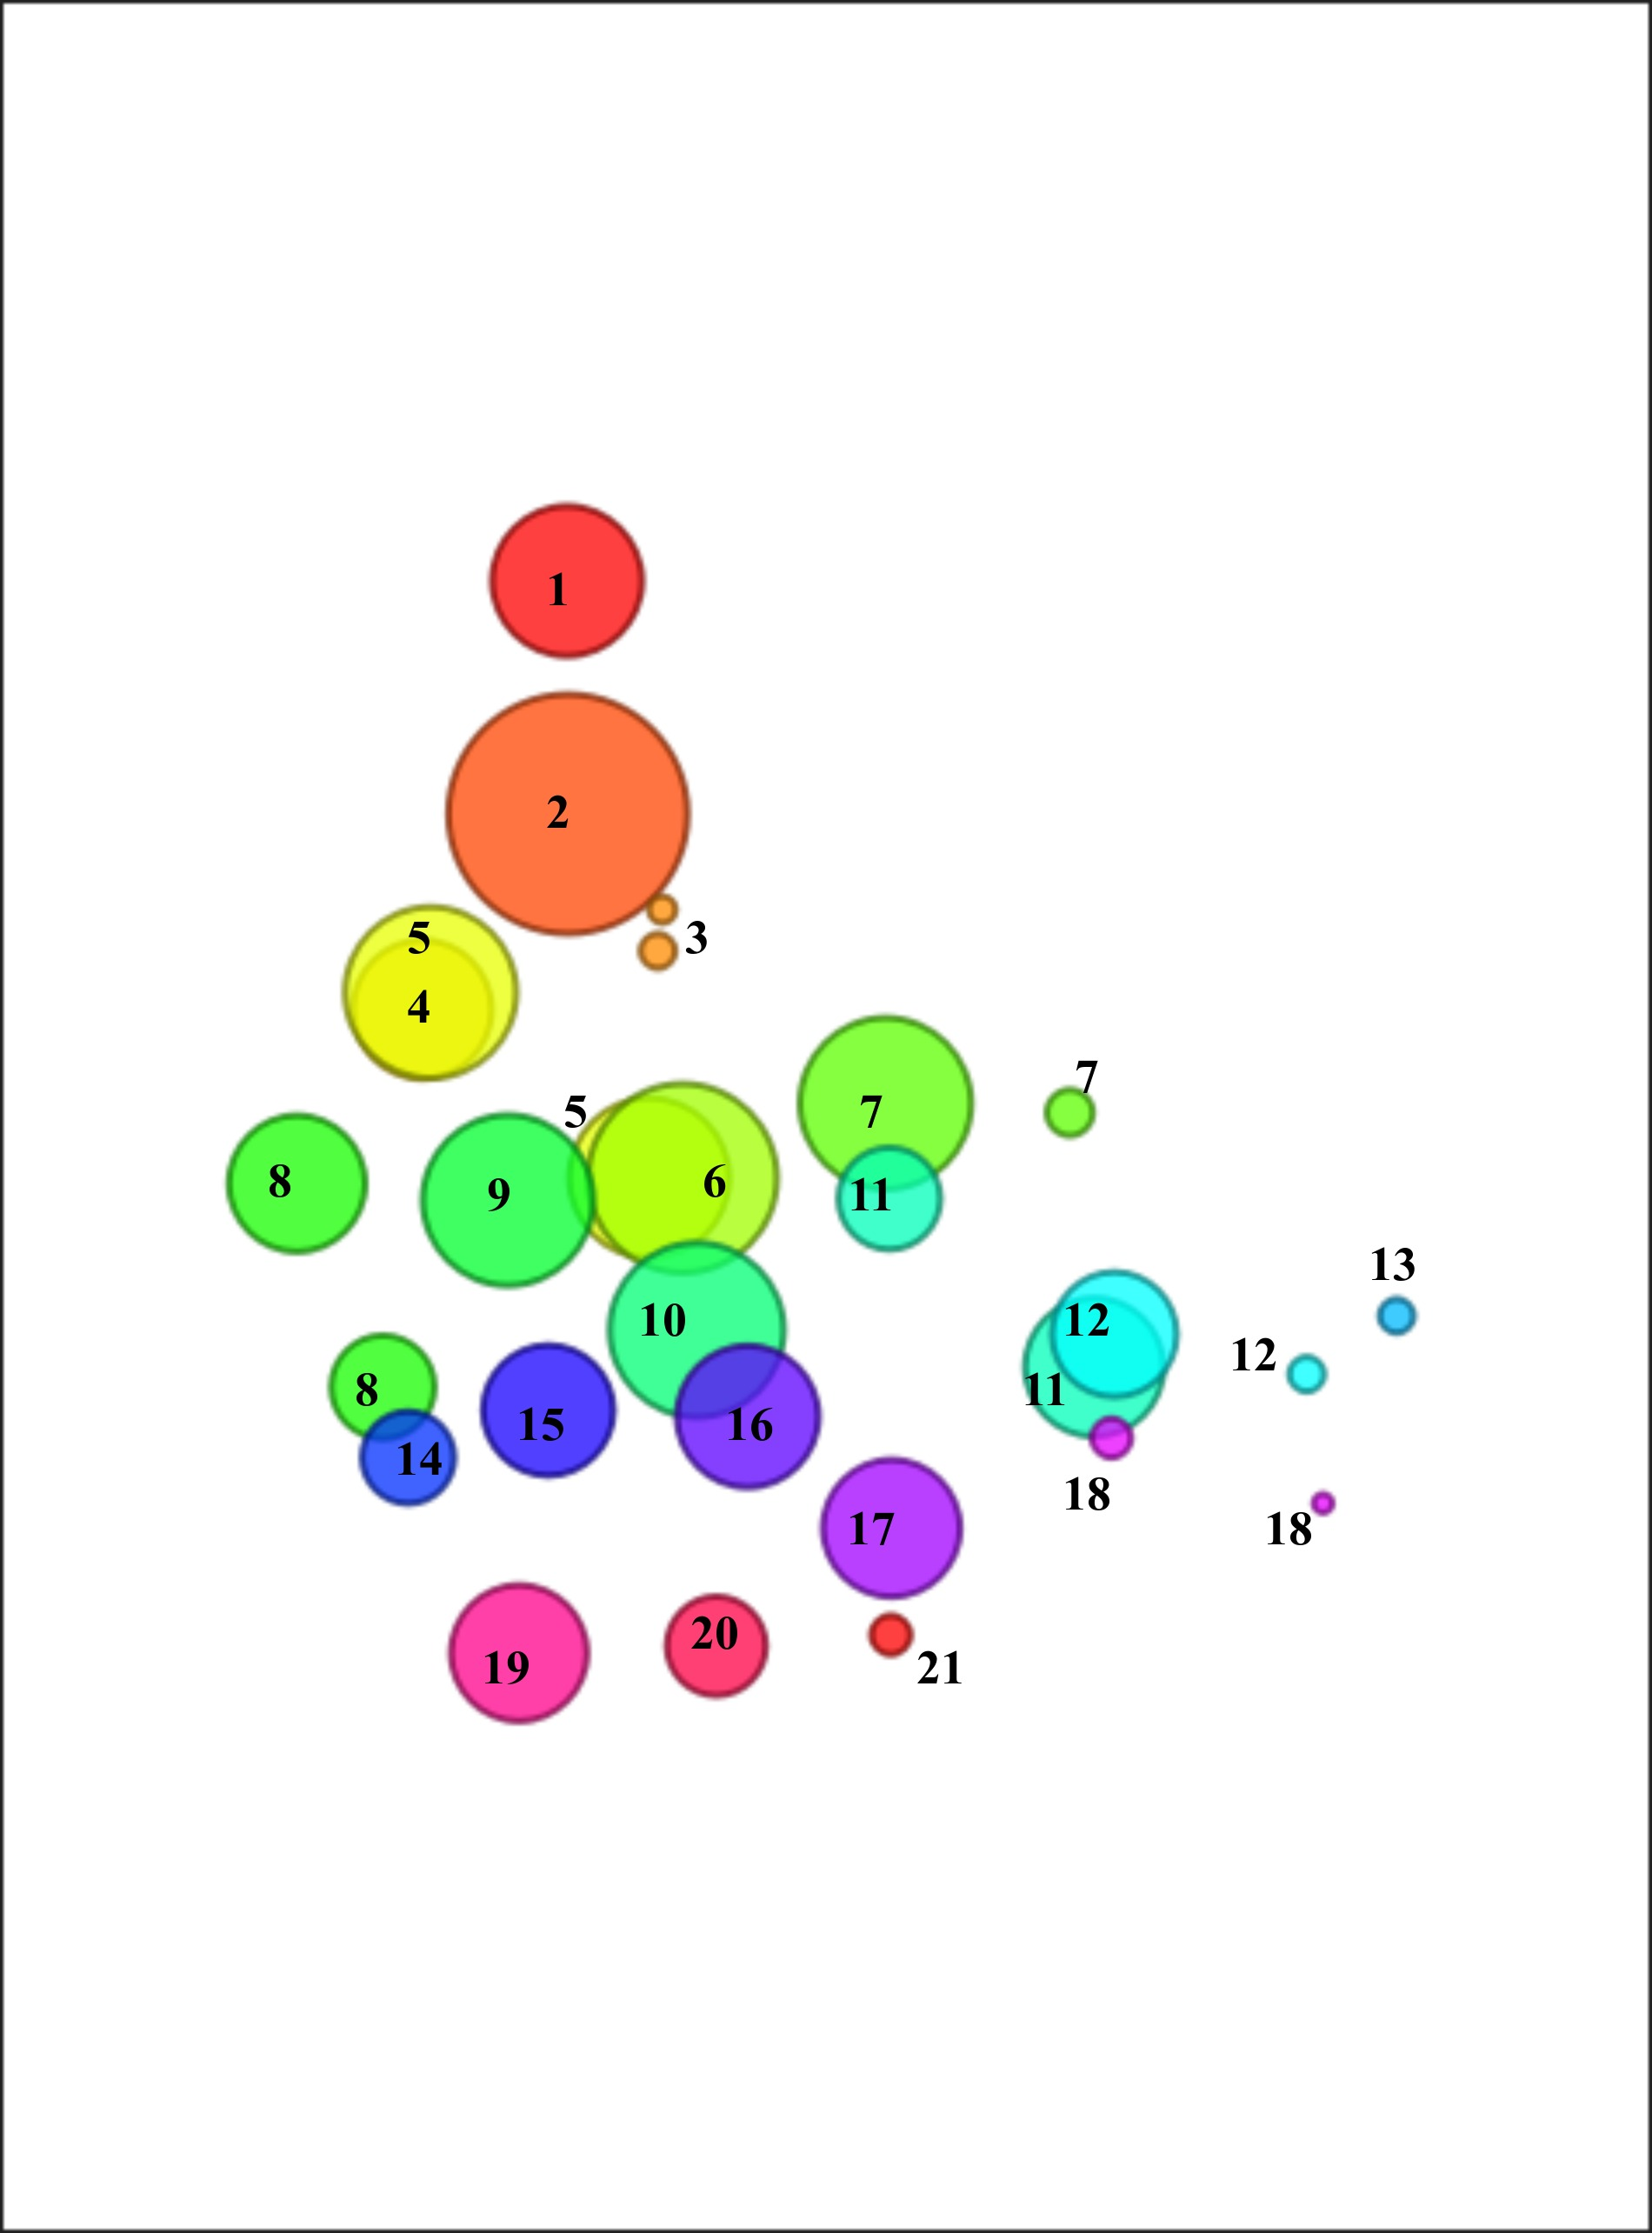
\includegraphics[width=0.7\columnwidth]{figs/engine-block-clusters-tf.jpg}
    \caption{Volume exploration space for the engine block dataset. Method parameters setup: transfer function $=\{$intensity, skewness, gradient magnitude and variance$\}$; $minPts = 4$;  $\varepsilon = 0.35$; and $\alpha = 0.85$.}
    \label{fig:engine-block-clusters-tf}
\end{figure}

\begin{figure}[htb!]
    \centering
    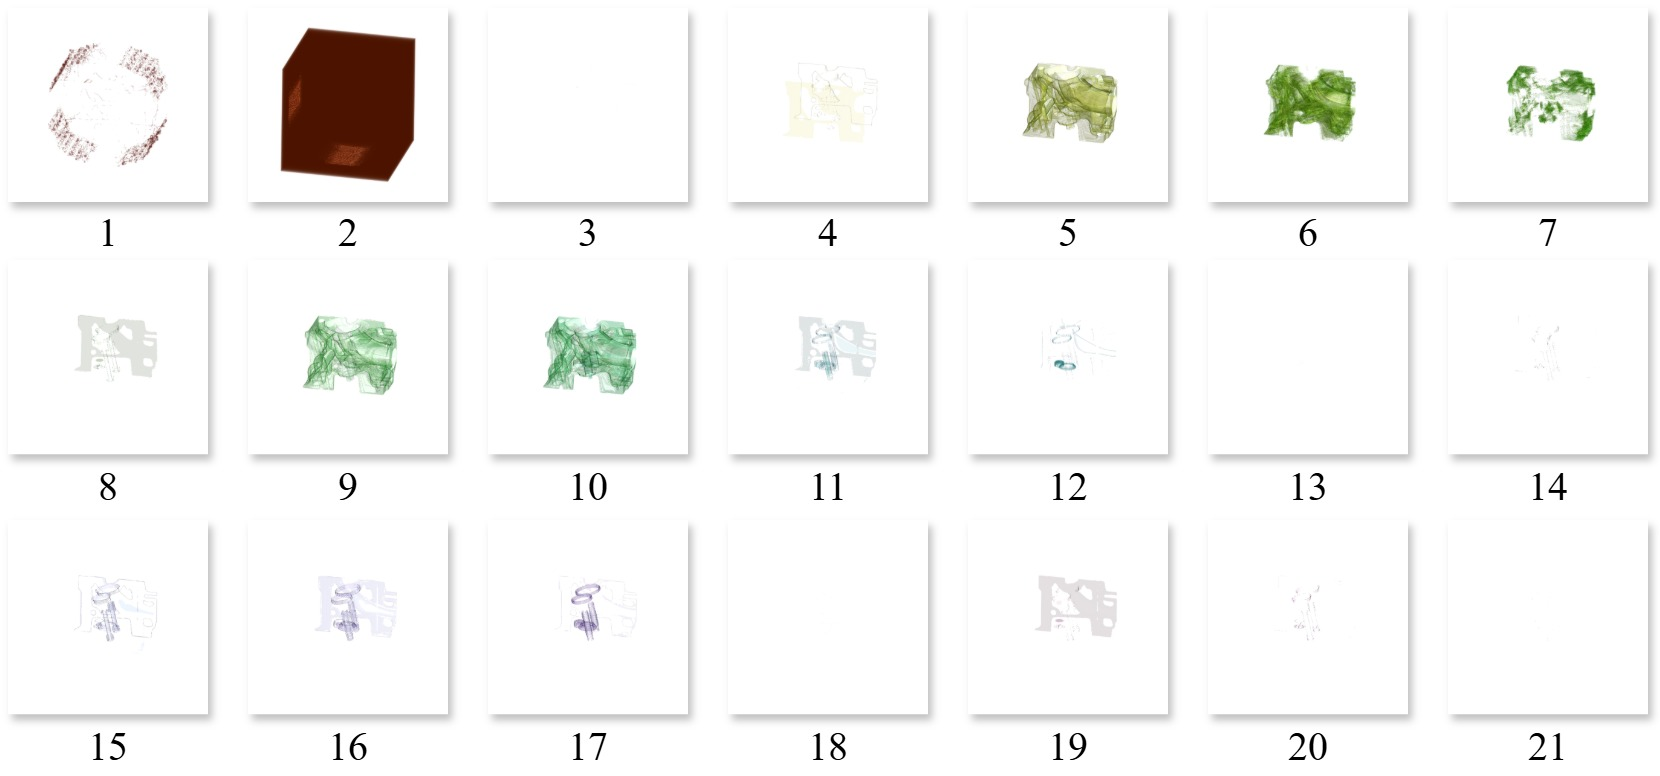
\includegraphics[width=\columnwidth]{figs/engine-block-clusters.jpg}
    \caption{Rendered volume classification details for the engine block dataset. Method parameters setup: transfer function  $=\{$intensity, skewness, gradient magnitude and variance$\}$; $minPts = 4$; $\varepsilon = 0.35$; and $\alpha = 0.85$.}
    \label{fig:engine-block-clusters}
\end{figure}

The rankings of attributes for the engine block dataset are shown in Table~\ref{tab:feature-ranking-for-engine-block}. We obtained the best results with the one based on the correlation coefficient measure.

\begin{table}[htb!]
    \caption{Rankings of volume data attributes for the engine block dataset.}
    \label{tab:feature-ranking-for-engine-block}
    \centering
    \begin{tabular}{@{}c>{\centering\arraybackslash}m{0.27\columnwidth}>{\centering\arraybackslash}m{0.27\columnwidth}>{\centering\arraybackslash}m{0.27\columnwidth}@{}}
        \toprule
         \textbf{$\#$} & \textbf{Least Squares Regression Error} & \textbf{Maximal Information Compression Index} & \textbf{Correlation Coefficient}\\
        \midrule
        $1$ & Intensity &  Intensity &  Intensity \\
        \hline
        $2$ & Energy &  Variance &  Skewness \\
        \hline
        $3$ & Inertia &  Absolute deviation & Gradient Magnitude \\
        \hline
        $4$ & Entropy &  Energy &  Variance \\
        \hline
        $5$ & Skewness &  Contrast &  Laplacian Magnitude \\
        \hline
        $6$ & Mean &  Entropy &  Entropy \\
        \hline
        $7$ & Absolute deviation &  Gradient Magnitude &  Energy \\
        \hline
        $8$ & Laplacian Magnitude &  Inertia &  Inertia \\
        \hline
        $9$ & Kurtosis &  Kurtosis &  Standard deviation \\
        \hline
        $10$ & Standard deviation &  Laplacian Magnitude &  Mean \\
        \hline
        $11$ & Gradient Magnitude &  Mean &  Kurtosis \\
        \hline
        $12$ & Contrast &  Skewness &  Absolute deviation \\
        \hline
        $13$ & Variance &  Standard deviation &  Contrast \\
        \bottomrule
    \end{tabular}
\end{table}

A volume exploration simulation is demonstrated in Fig.~\ref{fig:engine-block-groups}. It reveals different engine block components. The process happens from the initial setup presented in Fig.~\ref{fig:engine-block-clusters-tf}. 

\begin{figure}[htb!]
    \centering
    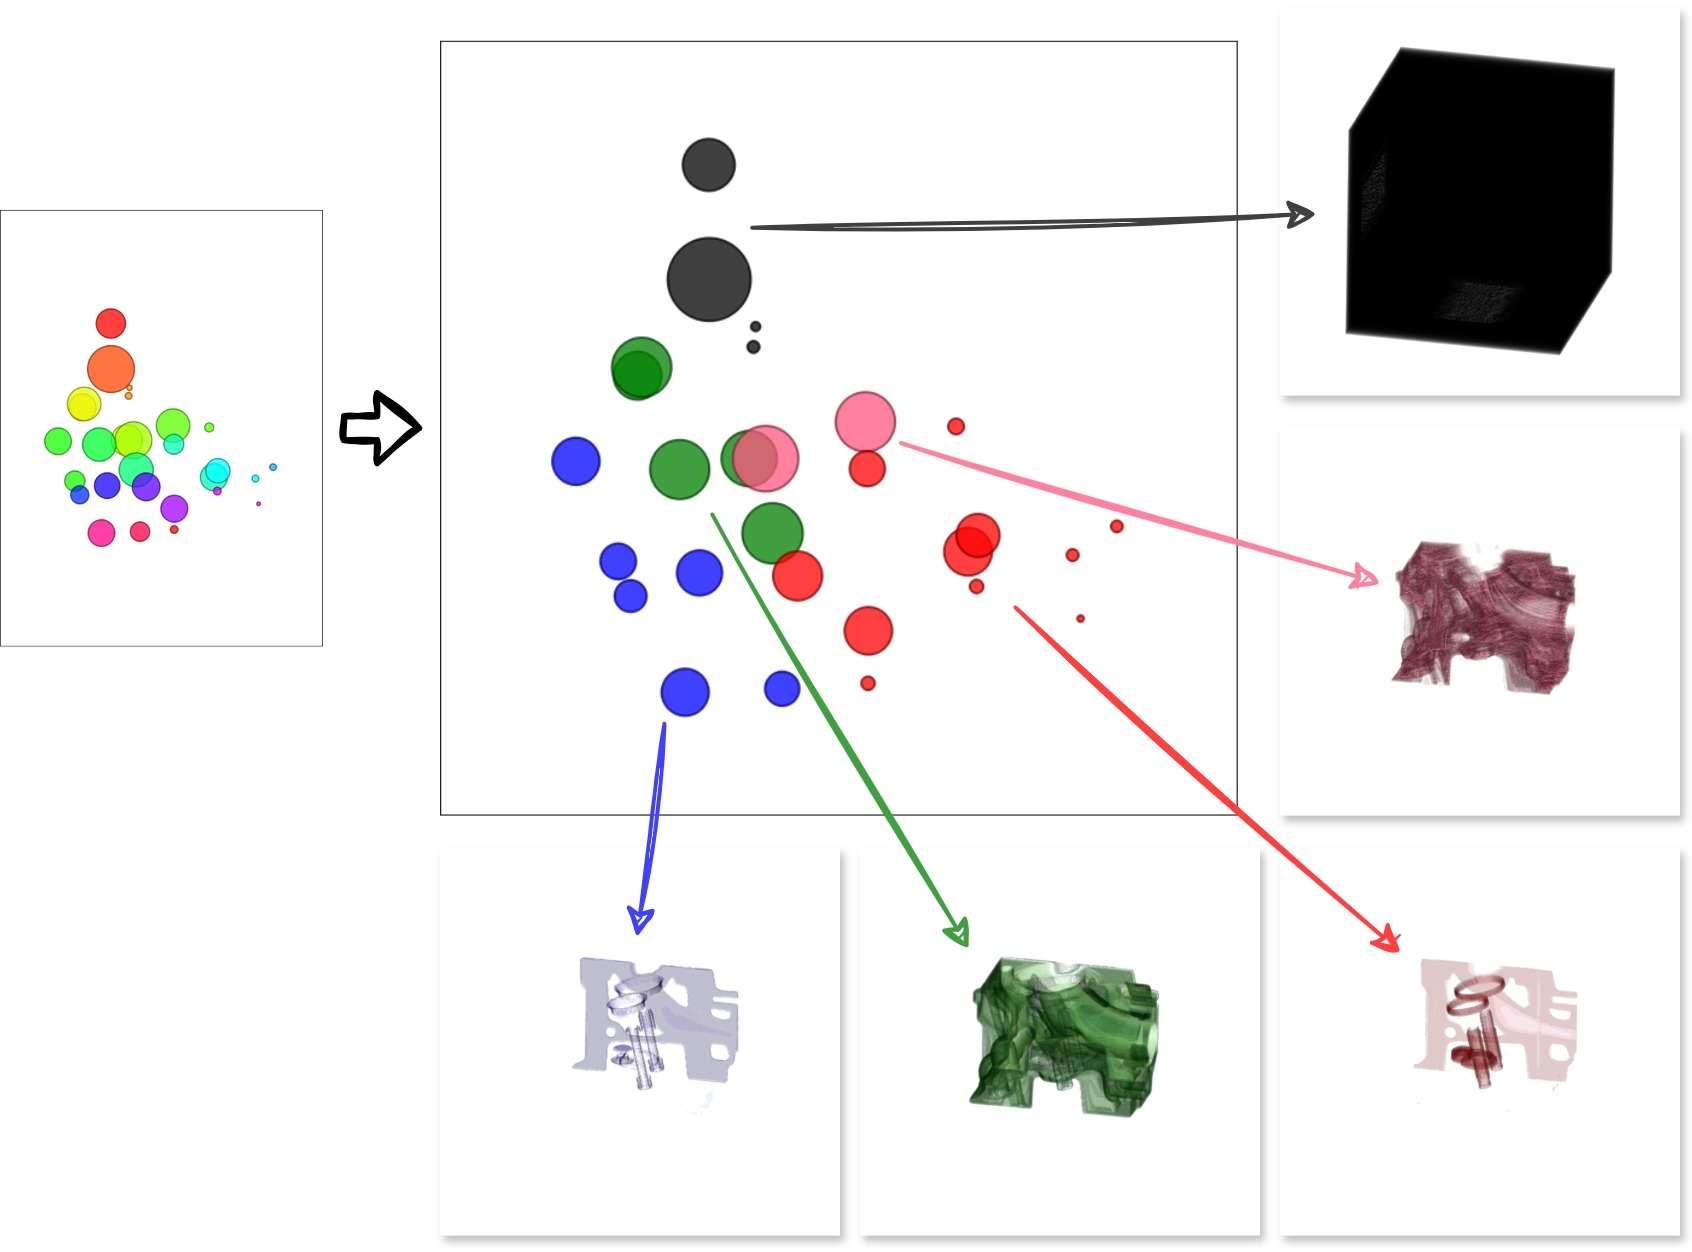
\includegraphics[width=\columnwidth]{figs/engine-block-groups.jpg}
    \caption{Visual analysis of user-refined transfer function design and volume classification for engine block datasets. The volume details are manually grouped from an empirical perspective. Method parameters setup: transfer function $=\{$intensity, skewness, gradient magnitude and variance$\}$; $minPts = 4$; $\varepsilon = 0.35$; and $\alpha = 0.85$.}
    \label{fig:engine-block-groups}
\end{figure}



\subsubsection{Knees dataset}
\label{subsubsect:knees-dataset}
A preliminary volume classification for knees datasets is presented in Fig.~\ref{fig:knees-tf-clusters} and the related rendered details in Fig.~\ref{fig:knees-clusters}. The method parameters are set as follows:  TF $=\{$intensity,  variance, absolute deviation, energy and contrast$\}$; $minPts = 4$; $\varepsilon = 0.35$; and $\alpha = 0.9$. 


\begin{figure}[htb!]
    \centering
    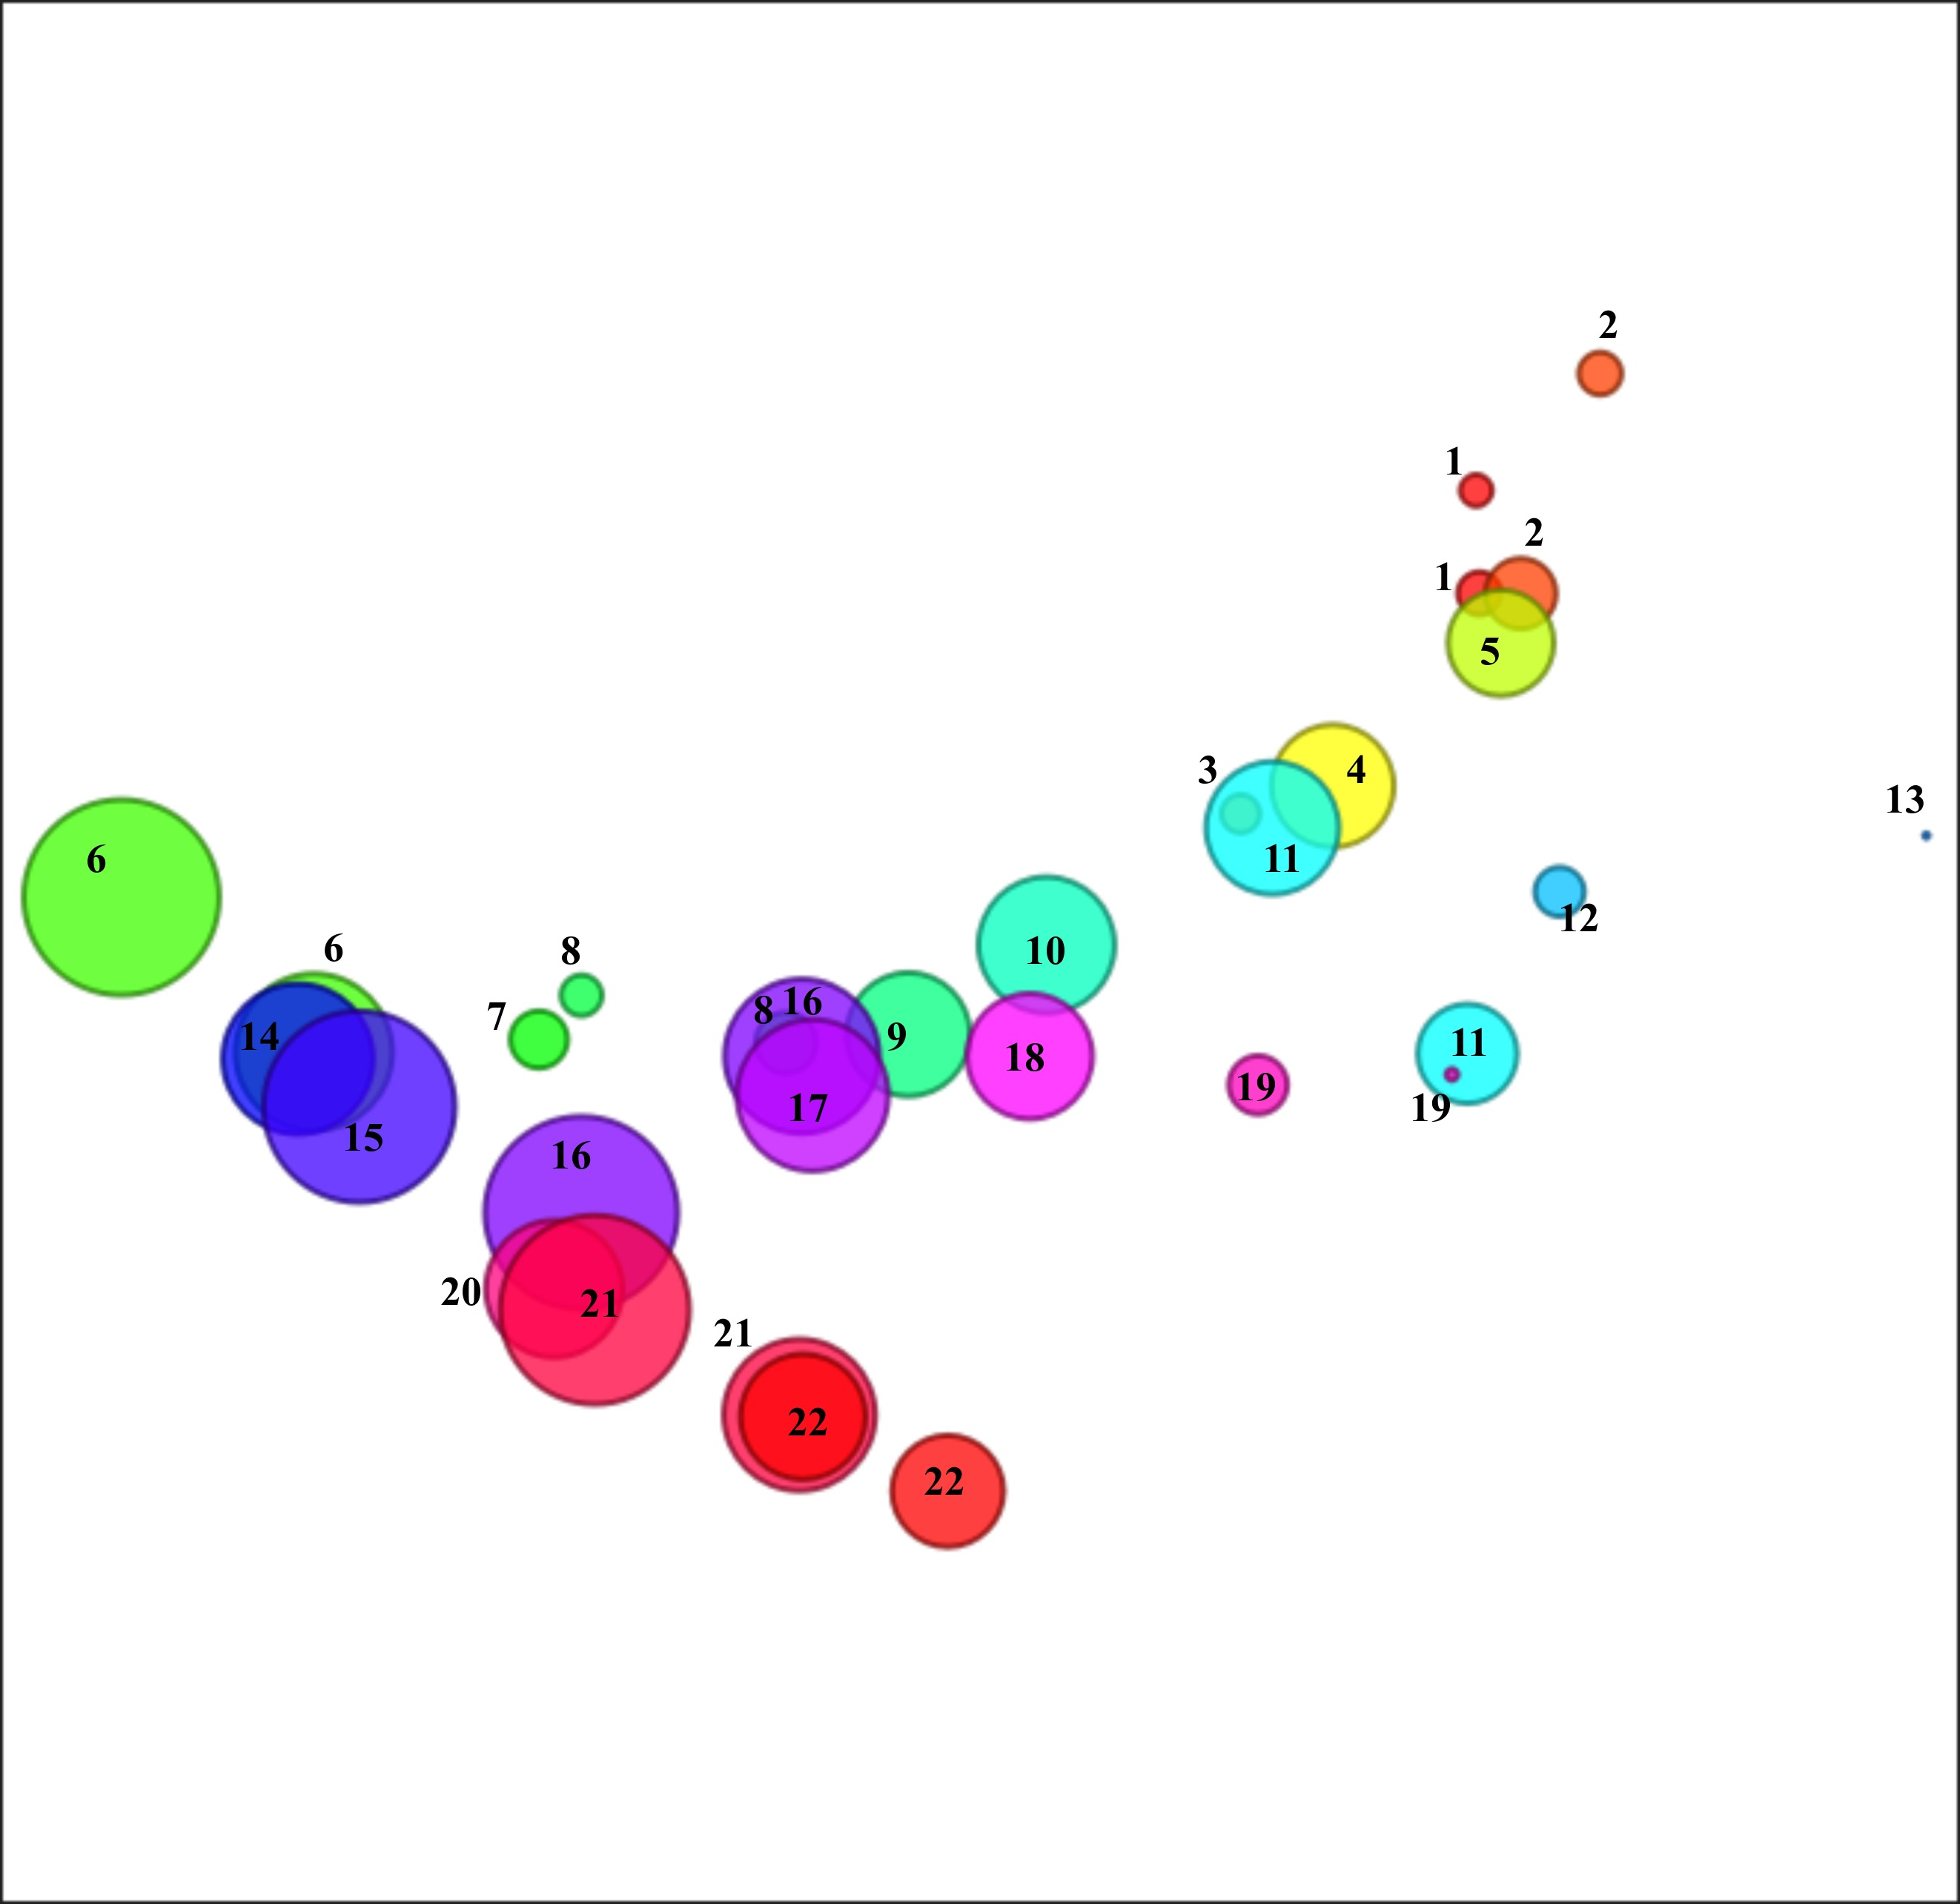
\includegraphics[width=0.7\columnwidth]{figs/knees-clusters-tf.jpg} 
     \caption{Volume exploration space for the knees dataset. Method parameters setup: transfer function $=\{$intensity,  variance, absolute deviation, energy and contrast$\}$; $minPts = 4$; $\varepsilon = 0.35$; and $\alpha = 0.9$.}
    \label{fig:knees-tf-clusters}
\end{figure}

\begin{figure}[htb!]
    \centering
    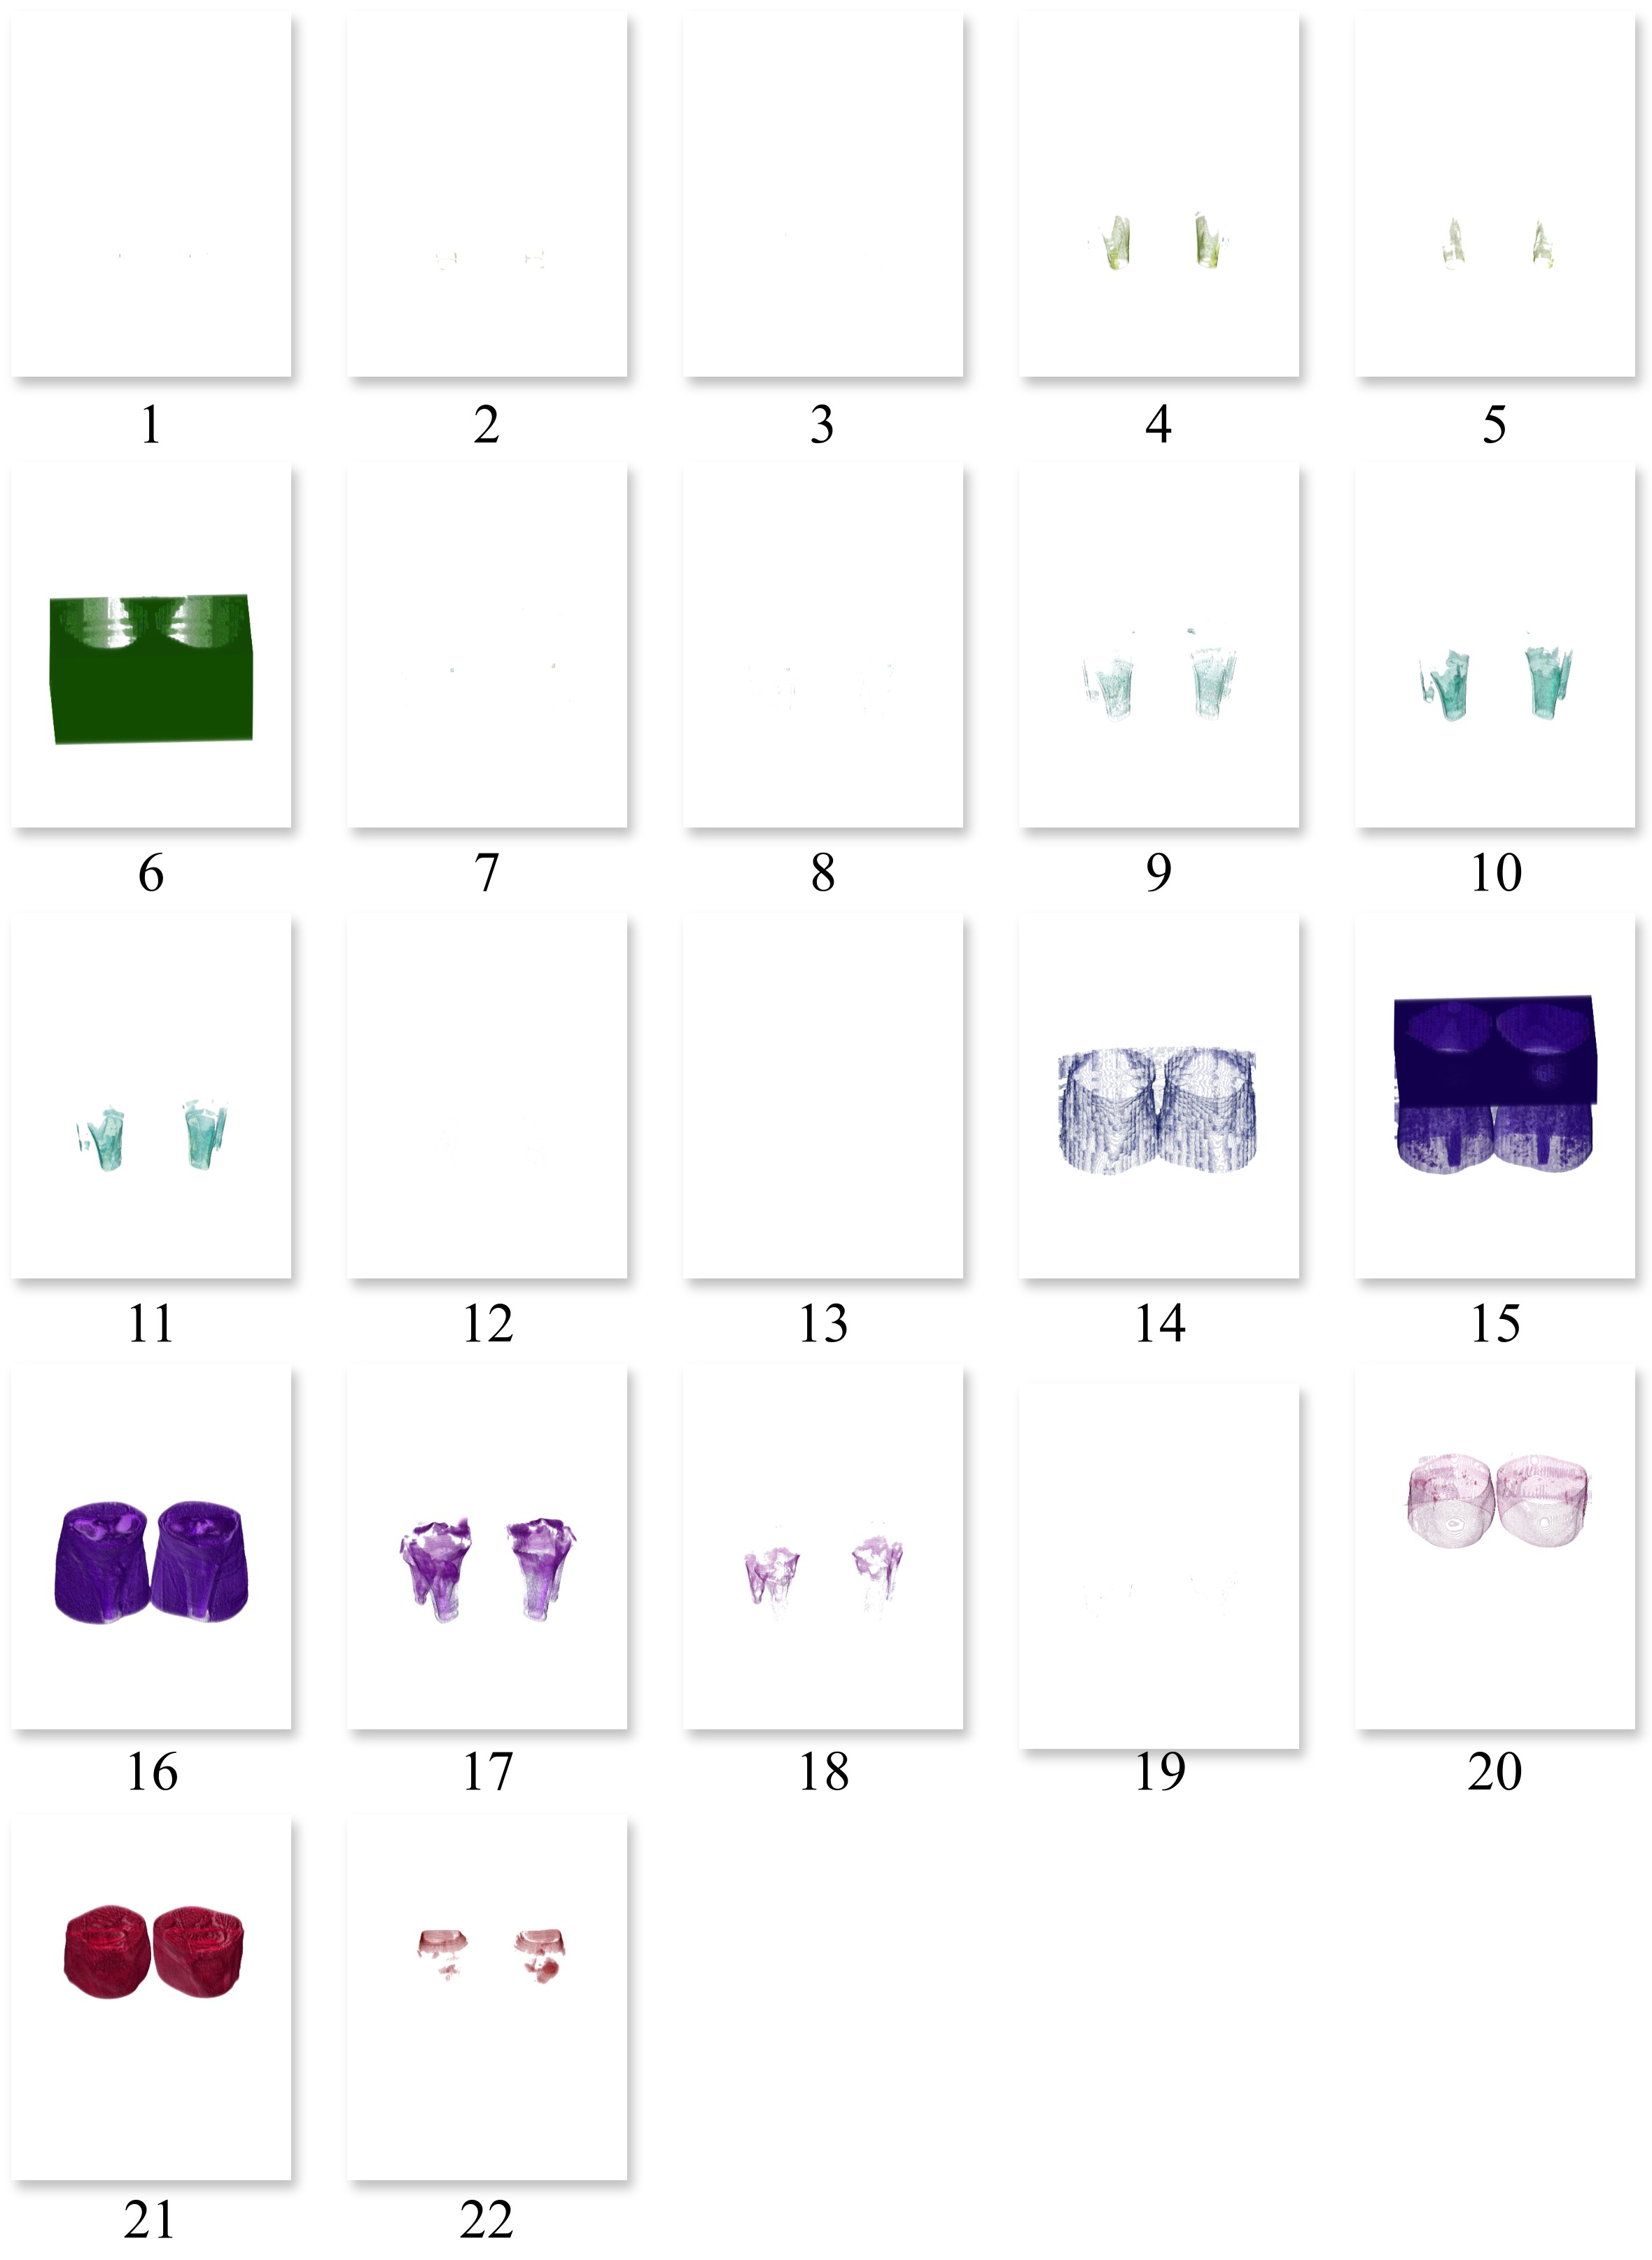
\includegraphics[width=\columnwidth]{figs/knees-clusters.jpg} 
     \caption{Rendered volume classification details for the knees dataset. Method parameters setup: transfer function $=\{$intensity,  variance, absolute deviation, energy and contrast$\}$; $minPts = 4$; $\varepsilon = 0.35$; and $\alpha = 0.9$.}
    \label{fig:knees-clusters}
\end{figure}

Table~\ref{tab:feature-ranking-for-tooth} presents the rankings generated for the tooth dataset.  We use the MICI measure ranking for the TF definition.

\begin{table}[htb!]
    \caption{Rankings of volume data attributes for the knees dataset.}
    \label{tab:feature-ranking-for-knees}
    \centering
    \begin{tabular}{@{}c>{\centering\arraybackslash}m{0.27\columnwidth}>{\centering\arraybackslash}m{0.27\columnwidth}>{\centering\arraybackslash}m{0.27\columnwidth}@{}}
        \toprule
         \textbf{$\#$} & \textbf{Least Squares Regression Error} & \textbf{Maximal Information Compression Index} & \textbf{Correlation Coefficient}\\
        \midrule
        $1$ & Intensity &  Intensity &  Intensity \\
        \hline
        $2$ & Entropy &  Variance &  Variance \\
        \hline
        $3$ & Energy &  Absolute deviation &  Skewness \\
        \hline
        $4$ & Inertia &  Energy &  Entropy \\
        \hline
        $5$ & Skewness &  Contrast &  Energy \\
        \hline
        $6$ & Laplacian Magnitude &  Entropy &  Inertia \\
        \hline
        $7$ & Mean &  Gradient Magnitude &  Standard deviation \\
        \hline
        $8$ & Absolute deviation &  Inertia &  Laplacian Magnitude \\
        \hline
        $9$ & Kurtosis &  Kurtosis &  Gradient Magnitude \\
        \hline
        $10$ & Standard deviation &  Laplacian Magnitude &  Kurtosis \\
        \hline
        $11$ & Gradient Magnitude &  Mean &  Absolute deviation \\
        \hline
        $12$ & Contrast &  Skewness &  Mean \\
        \hline
        $13$ & Variance &  Standard deviation &  Contrast \\
        \bottomrule
    \end{tabular}
\end{table}

By exploring the volume details, it is possible to group and identify bones and muscular structures. Fig.~\ref{fig:knees-groups} illustrates these structures, which include parts of the femur, tibia, patella, fibula, thigh muscles, and knee muscles.

\begin{figure}[htb!]
    \centering
    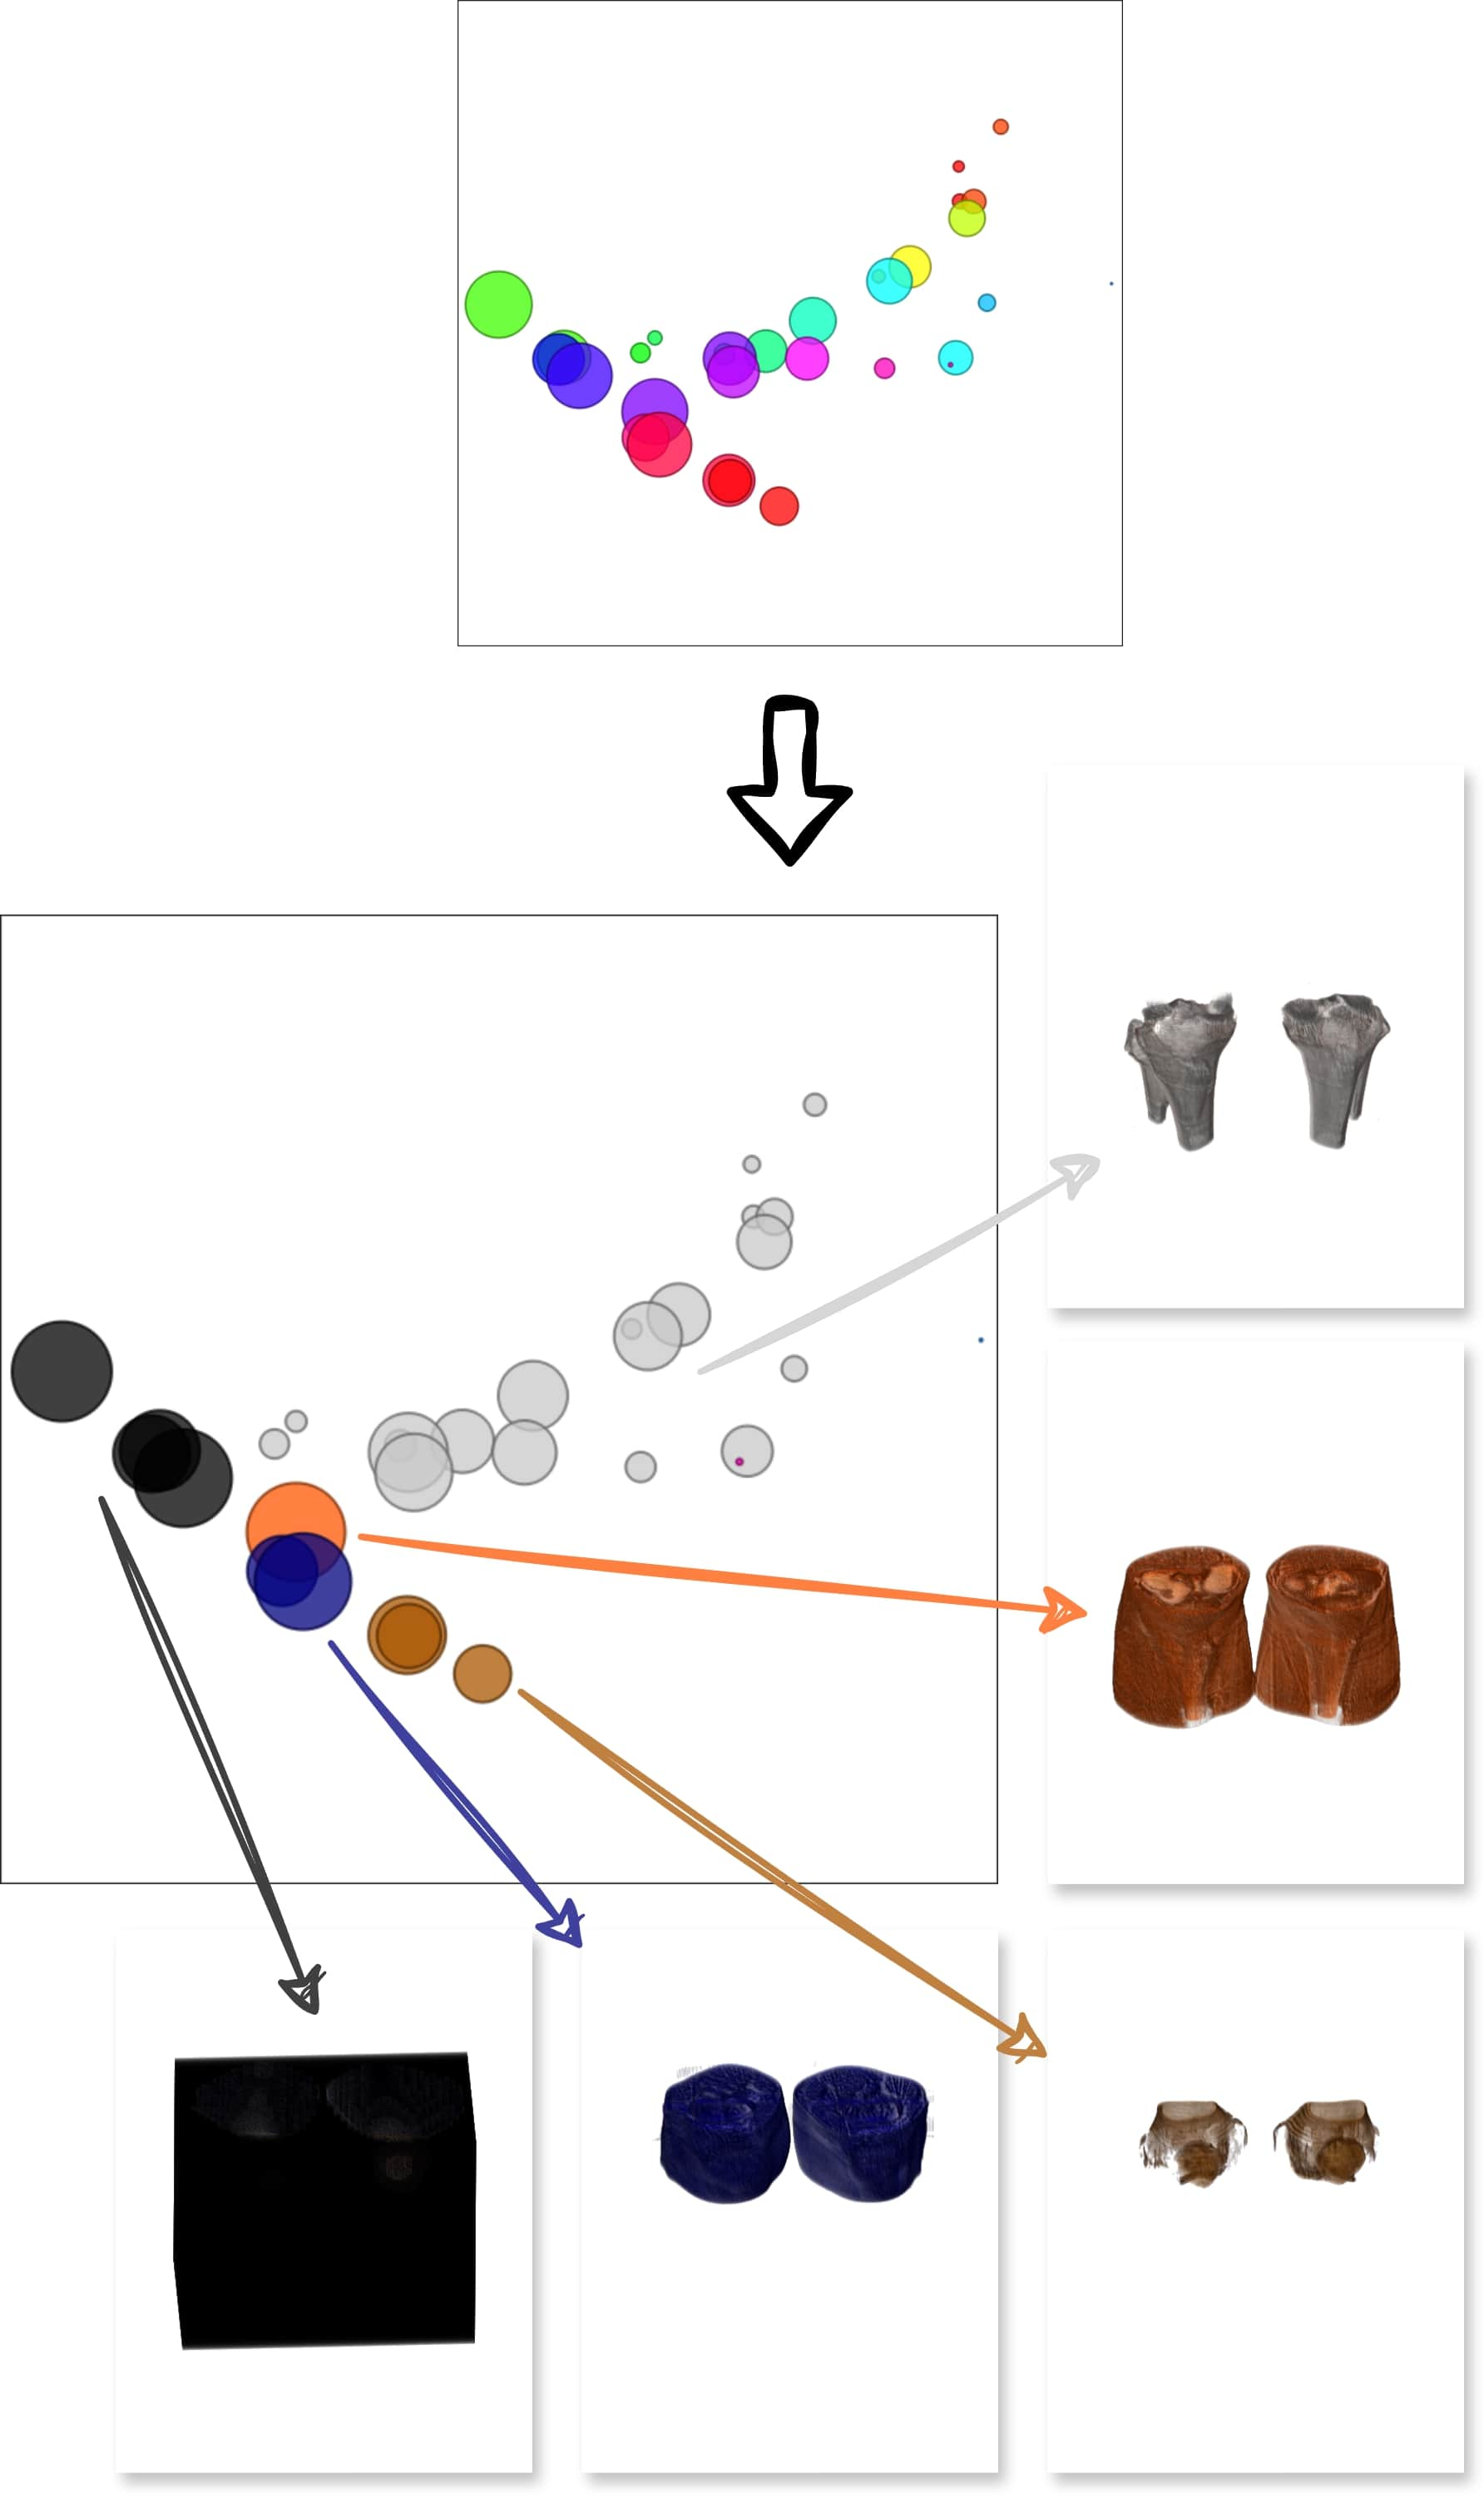
\includegraphics[width=\columnwidth]{figs/knees-groups.jpg}
    \caption{Visual analysis of user-refined transfer function design and volume classification for knees dataset. The volume details are manually grouped from an empirical perspective. Method parameters setup: transfer function $=\{$intensity,  variance, absolute deviation, energy and contrast$\}$; $minPts = 4$; $\varepsilon = 0.35$; and $\alpha = 0.9$.}
    \label{fig:knees-groups}
\end{figure}




\subsubsection{Tooth dataset}
\label{subsubsect:tooth-dataset}
Fig.~\ref{fig:tooth-clusters} presents  visualizations of a tooth dataset classification. The method parameters are set as follows:  TF $= \{$intensity, variance, absolute deviation, energy, contrast and entropy$\}$; $minPts = 4$; $\varepsilon = 0.23$; and $\alpha = 0.9$.

Table~\ref{tab:feature-ranking-for-tooth}  outlines the attribute dissimilarity rankings. The ranking based on the MICI measure is which one is chosen to support the TF definition. 

\begin{figure}[htb!]
    \centering
    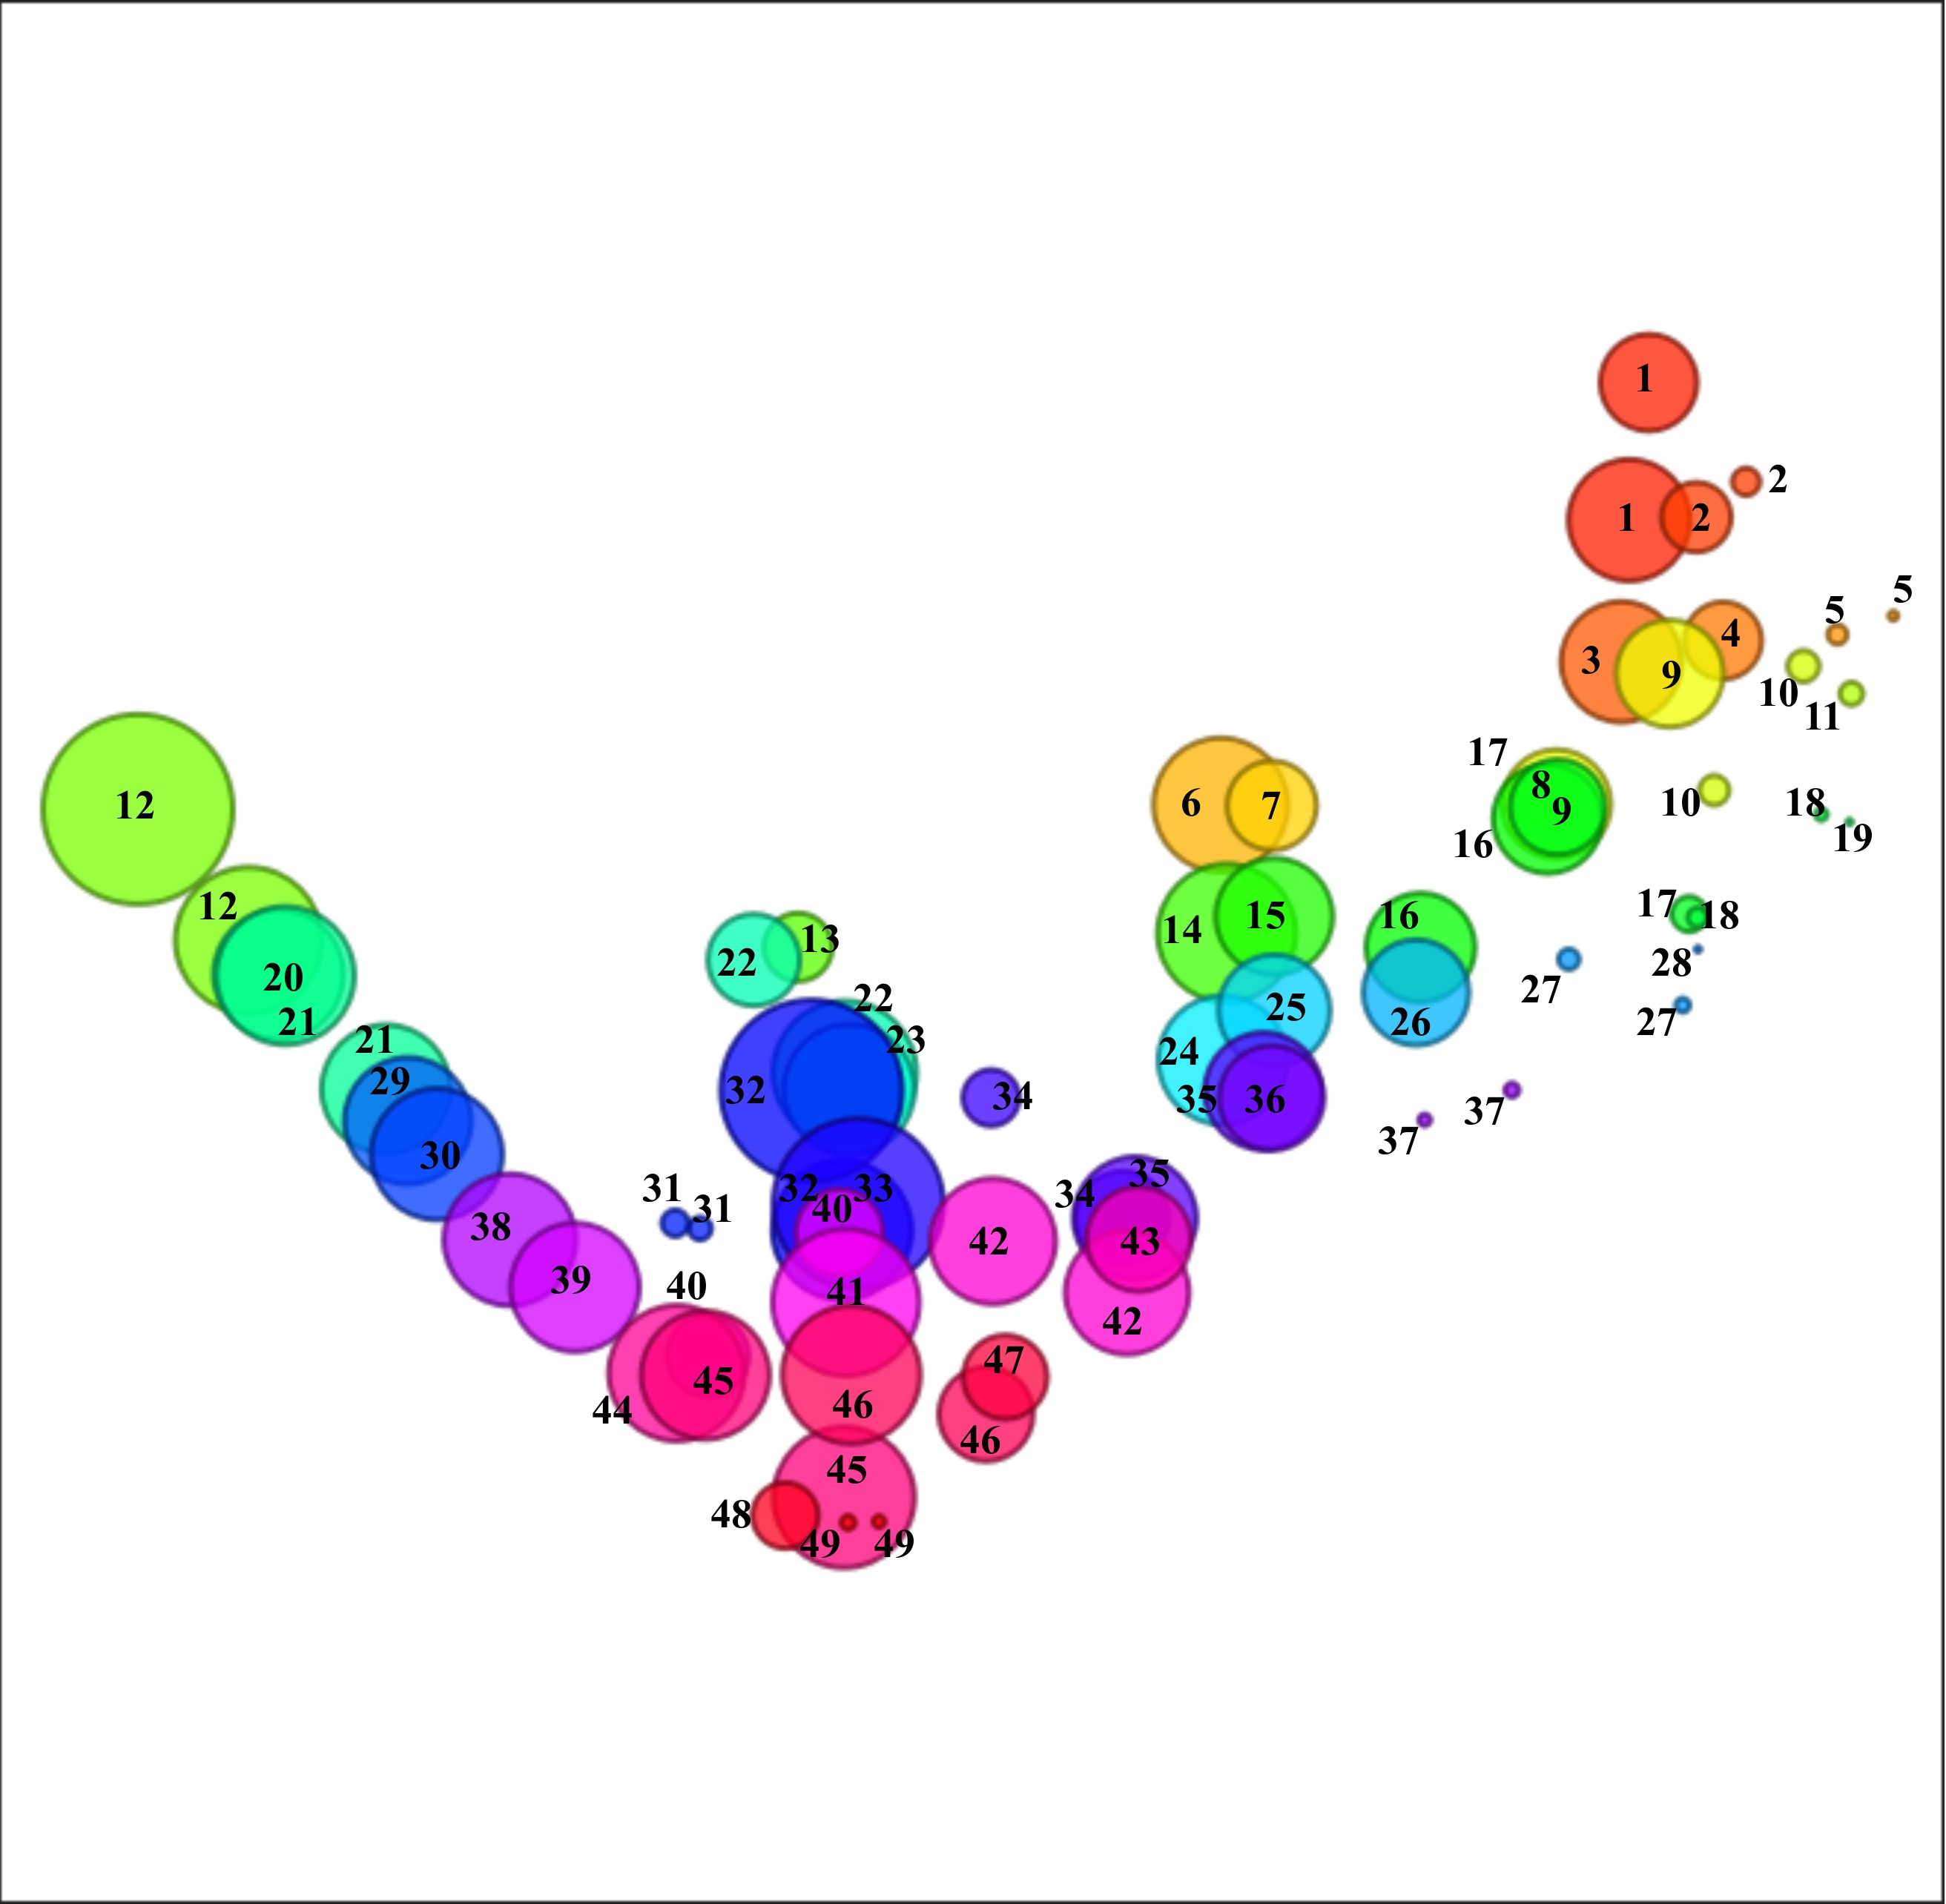
\includegraphics[width=0.7\columnwidth]{figs/tooth-clusters-tf.jpg} 
    \caption{Volume exploration space for the tooth dataset. Method parameters setup: transfer function $ =\{$intensity, variance, absolute deviation, energy, contrast and entropy$\}$; $minPts = 4$; $\varepsilon = 0.23$; and $\alpha = 0.9$.}
    \label{fig:tooth-clusters}
\end{figure}

\begin{figure}[htb!]
    \centering
    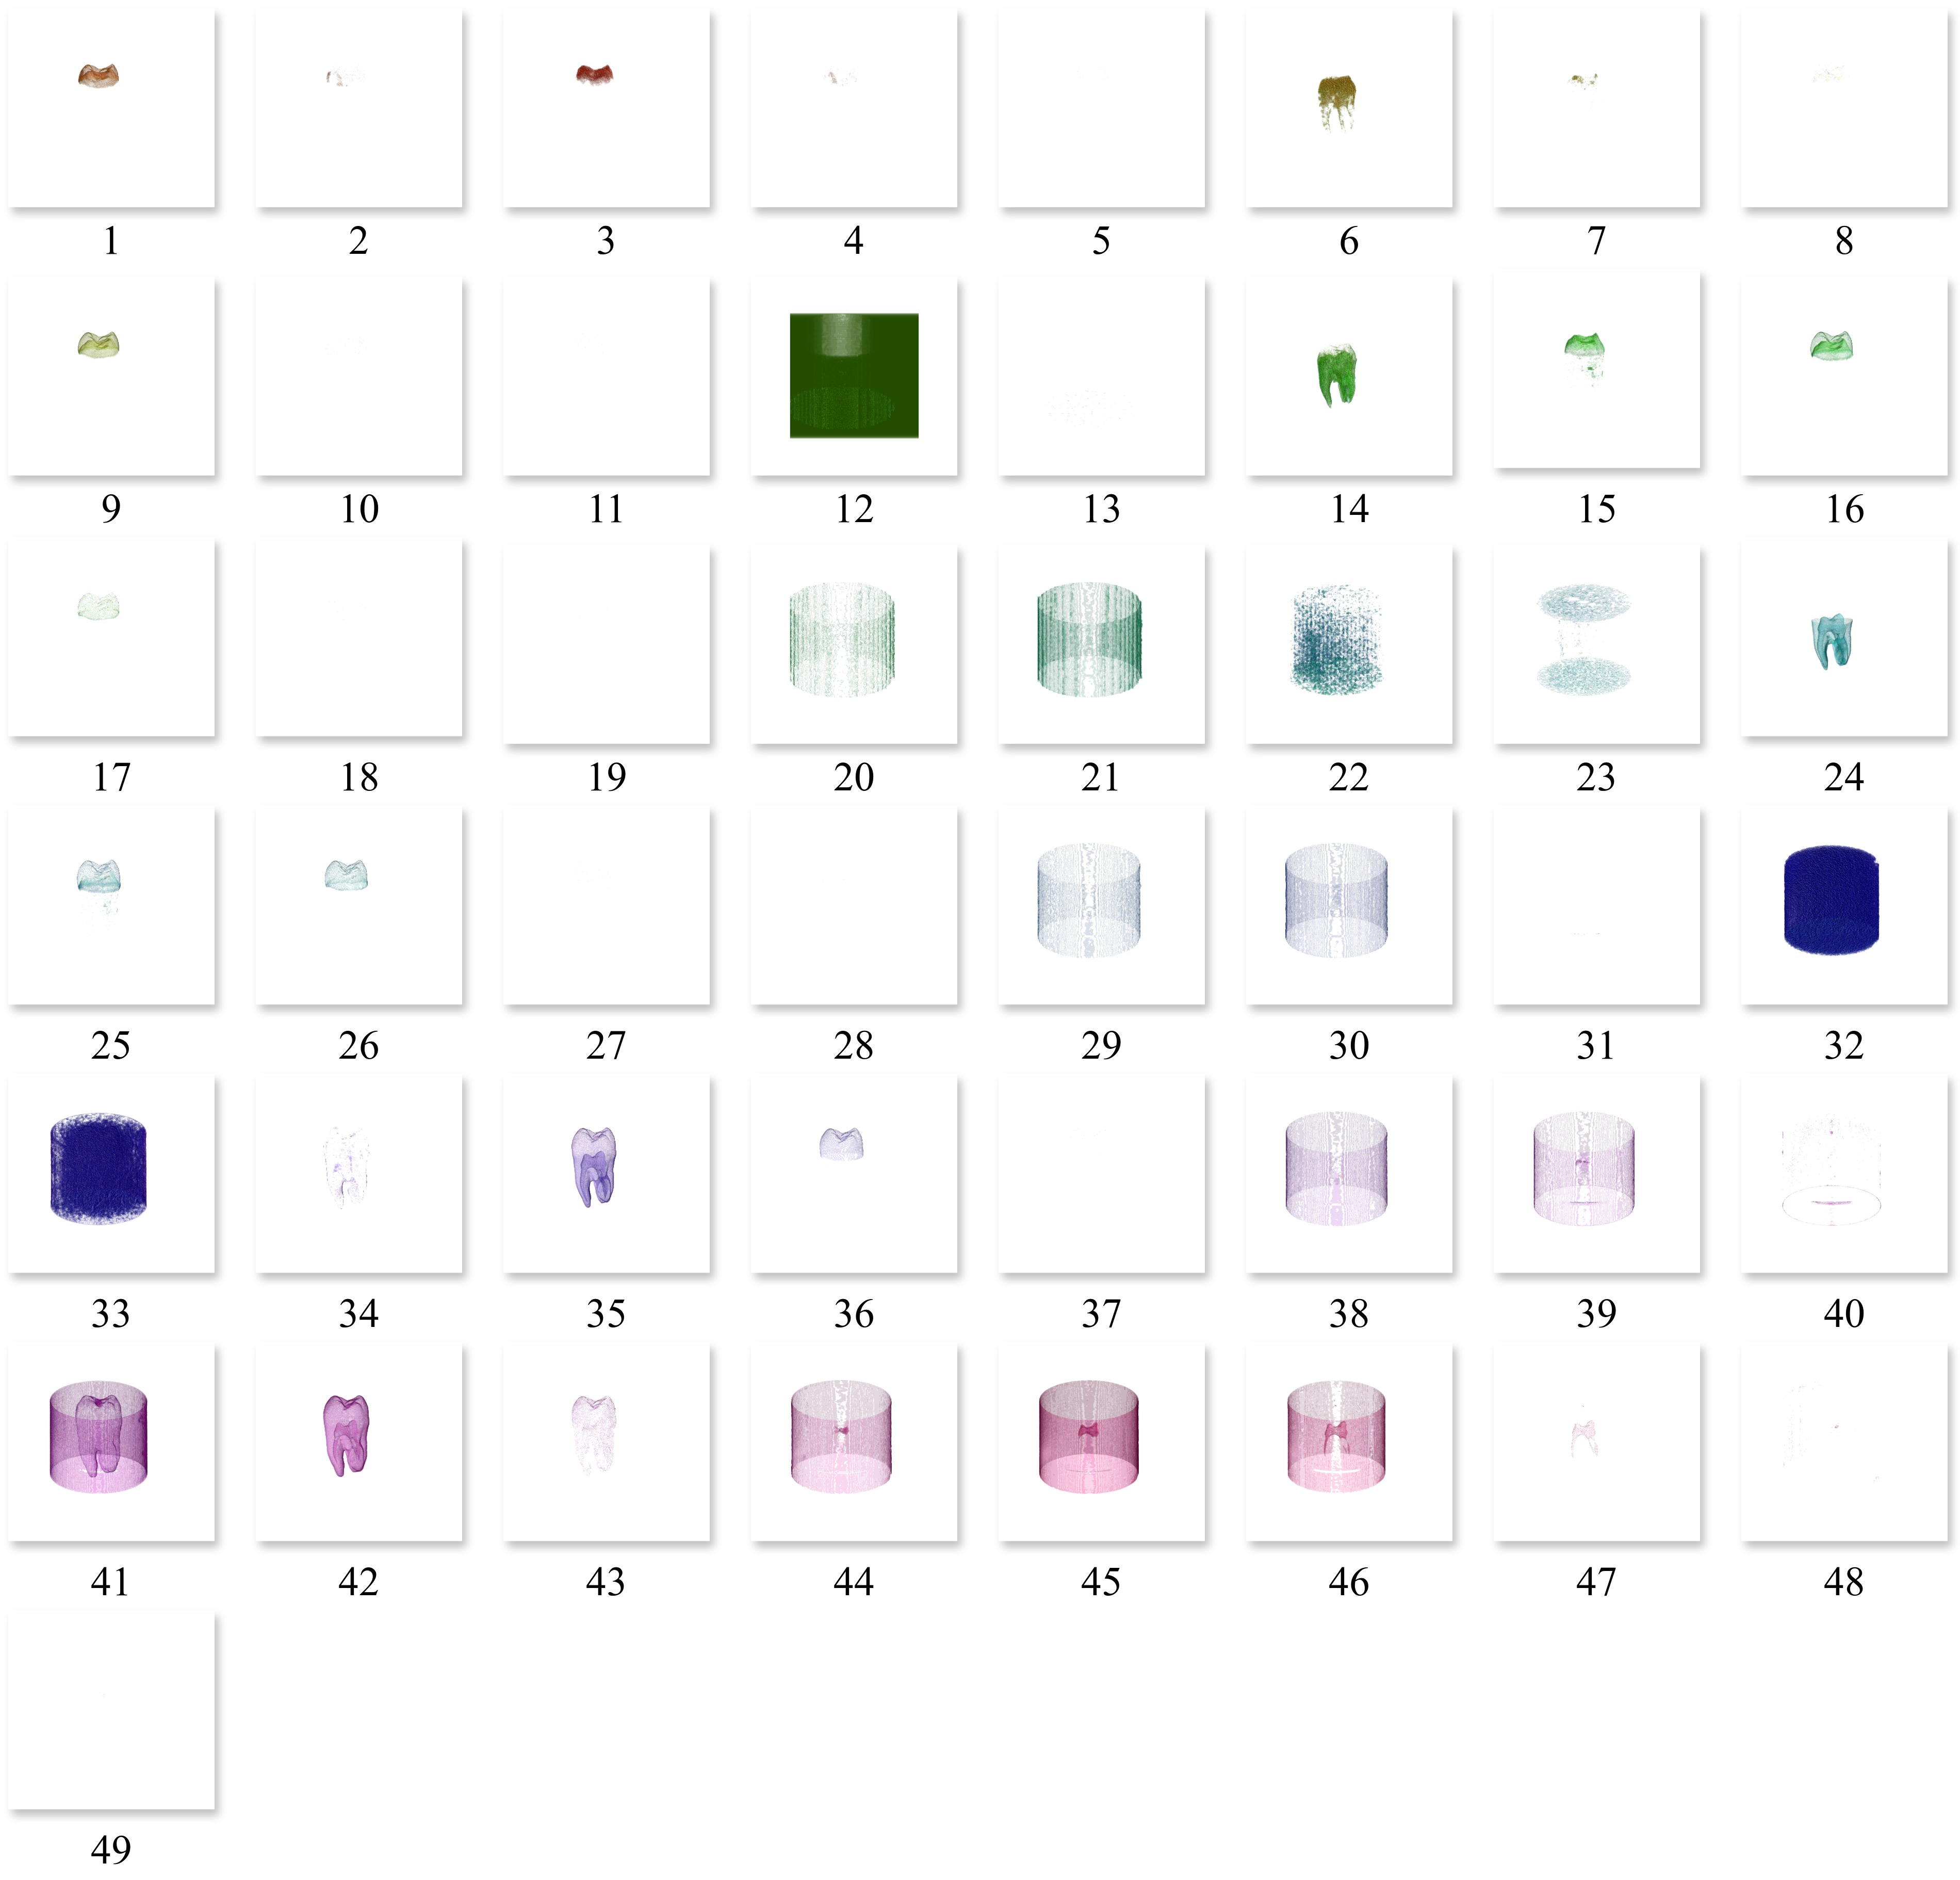
\includegraphics[width=\columnwidth]{figs/tooth-clusters.jpg} 
    \caption{Rendered volume classification details for the tooth dataset. The method parameters are set as follows: transfer function $ =\{$intensity, variance, absolute deviation, energy, contrast and entropy$\}$; $minPts = 4$; $\varepsilon = 0.23$; and $\alpha = 0.9$.}
    \label{fig:tooth-clusters}
\end{figure}


Manually generated groups of related tooth details are presented in Fig.~\ref{fig:tooth-groups}.  It shows several discernible structures, including the enamel, pulp, dentin, crown, the entire tooth, and the fluid in which it is immersed.

\begin{table}[htb!]
    \centering
    \caption{Rankings of volume data attributes for the tooth dataset.}
    \label{tab:feature-ranking-for-tooth}
    \begin{tabular}{@{}c>{\centering\arraybackslash}m{0.27\columnwidth}>{\centering\arraybackslash}m{0.27\columnwidth}>{\centering\arraybackslash}m{0.27\columnwidth}@{}}
        \toprule
         \textbf{$\#$} & \textbf{Least Square Regression Error} & \textbf{Maximal Information Compression Index} & \textbf{Correlation Coefficient}\\
        \midrule
        $1$ & Intensity &  Intensity &  Intensity \\
        \hline
        $2$ & Energy &  Variance &  Variance \\
        \hline
        $3$ & Inertia &  Absolute deviation &  Skewness \\
        \hline
        $4$ & Entropy &  Energy &  Gradient Magnitude \\
        \hline
        $5$ & Skewness &  Contrast &  Laplacian Magnitude \\
        \hline
        $6$ & Laplacian Magnitude &  Entropy &  Energy \\
        \hline
        $7$ & Mean &  Gradient Magnitude &  Inertia \\
        \hline
        $8$ & Absolute deviation &  Inertia &  Standard deviation \\
        \hline
        $9$ & Kurtosis &  Kurtosis &  Entropy \\
        \hline
        $10$ & Gradient Magnitude &  Laplacian Magnitude &  Kurtosis \\
        \hline
        $11$ & Standard deviation &  Mean &  Absolute deviation \\
        \hline
        $12$ & Contrast &  Skewness &  Mean \\
        \hline
        $13$ & Variance &  Standard deviation &  Contrast \\
        \bottomrule
    \end{tabular}
\end{table}

\begin{figure}[htb!]
    \centering
    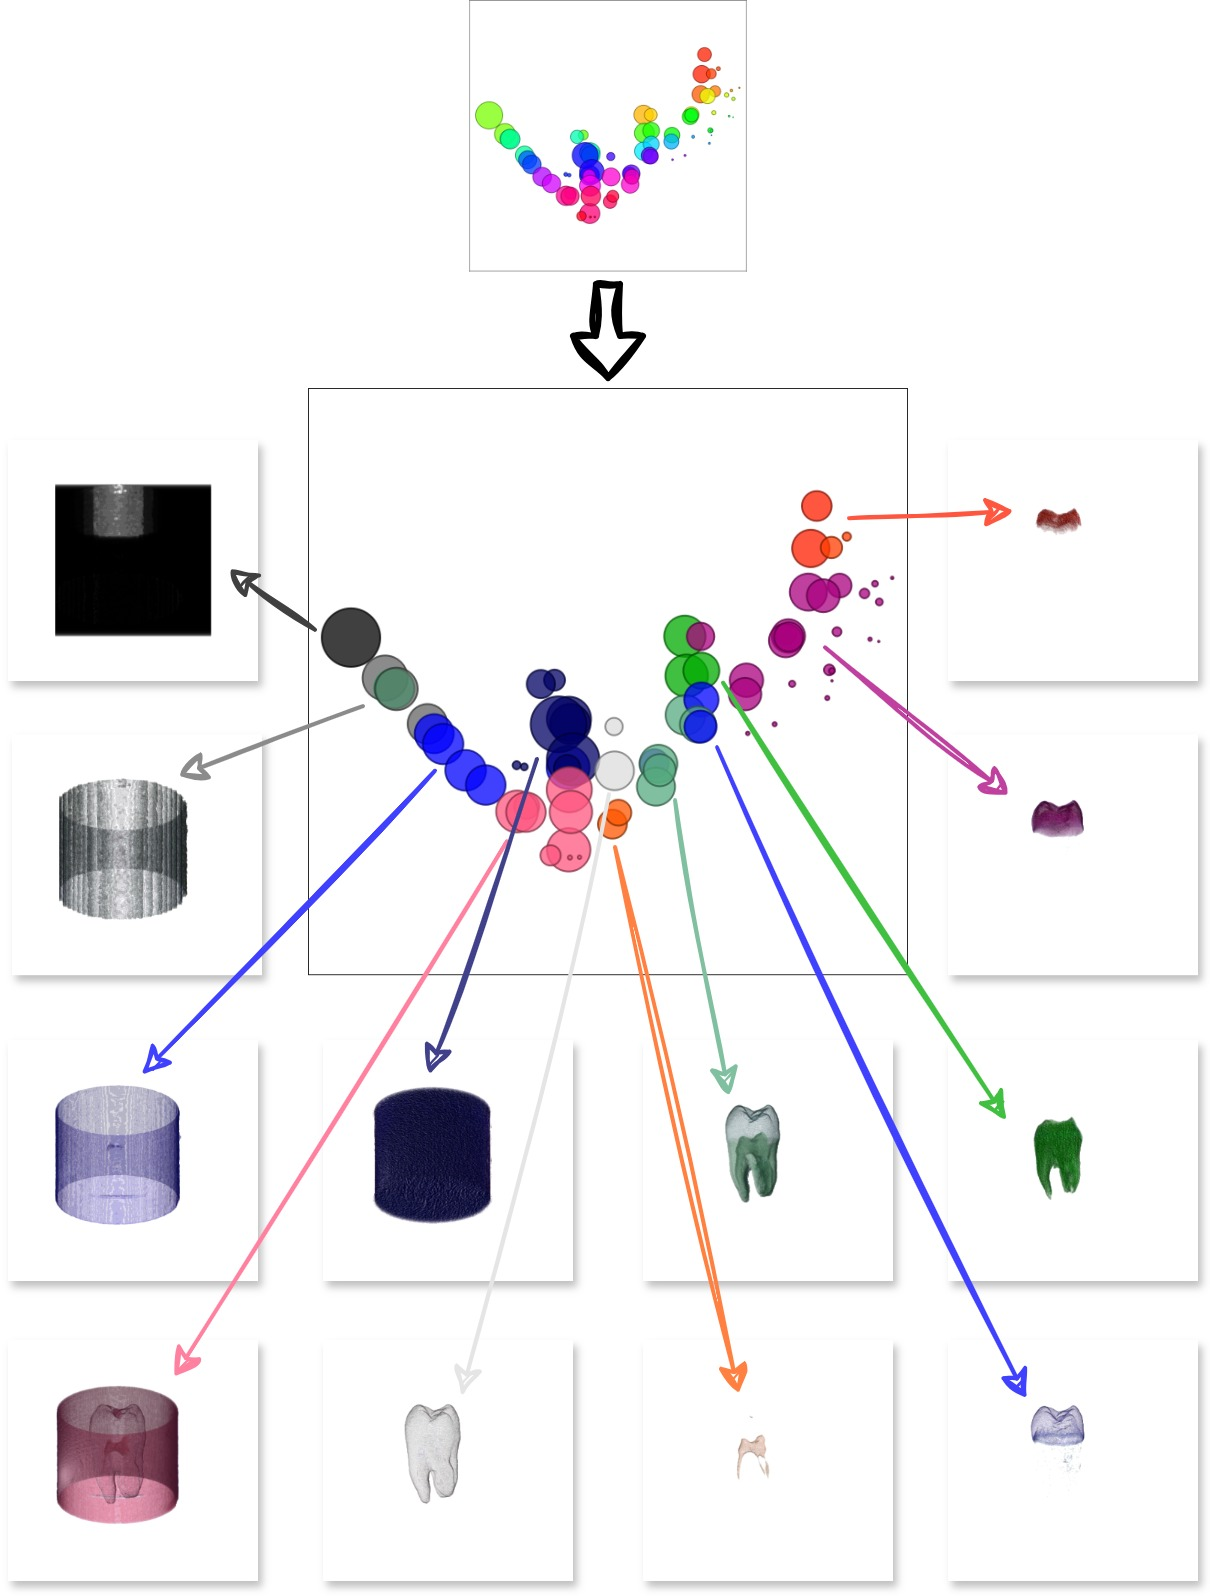
\includegraphics[width=\columnwidth]{figs/tooth-groups.jpg}
    \caption{Visual analysis of user-refined transfer function design and volume classification for tooth dataset. The volume details are manually grouped from an empirical perspective. The method parameters are set as follows: transfer function domain $ =\{$intensity, variance, absolute deviation, energy, contrast and entropy$\}$; $minPts = 4$; $\varepsilon = 0.23$; and $\alpha = 0.9$.}
    \label{fig:tooth-groups}
\end{figure}